\todo{im prinzip nur aus dem Manifesto abschreiben}
\chapter{Use Cases\label{chap:usecases}}
\begin{figure}[htbp]
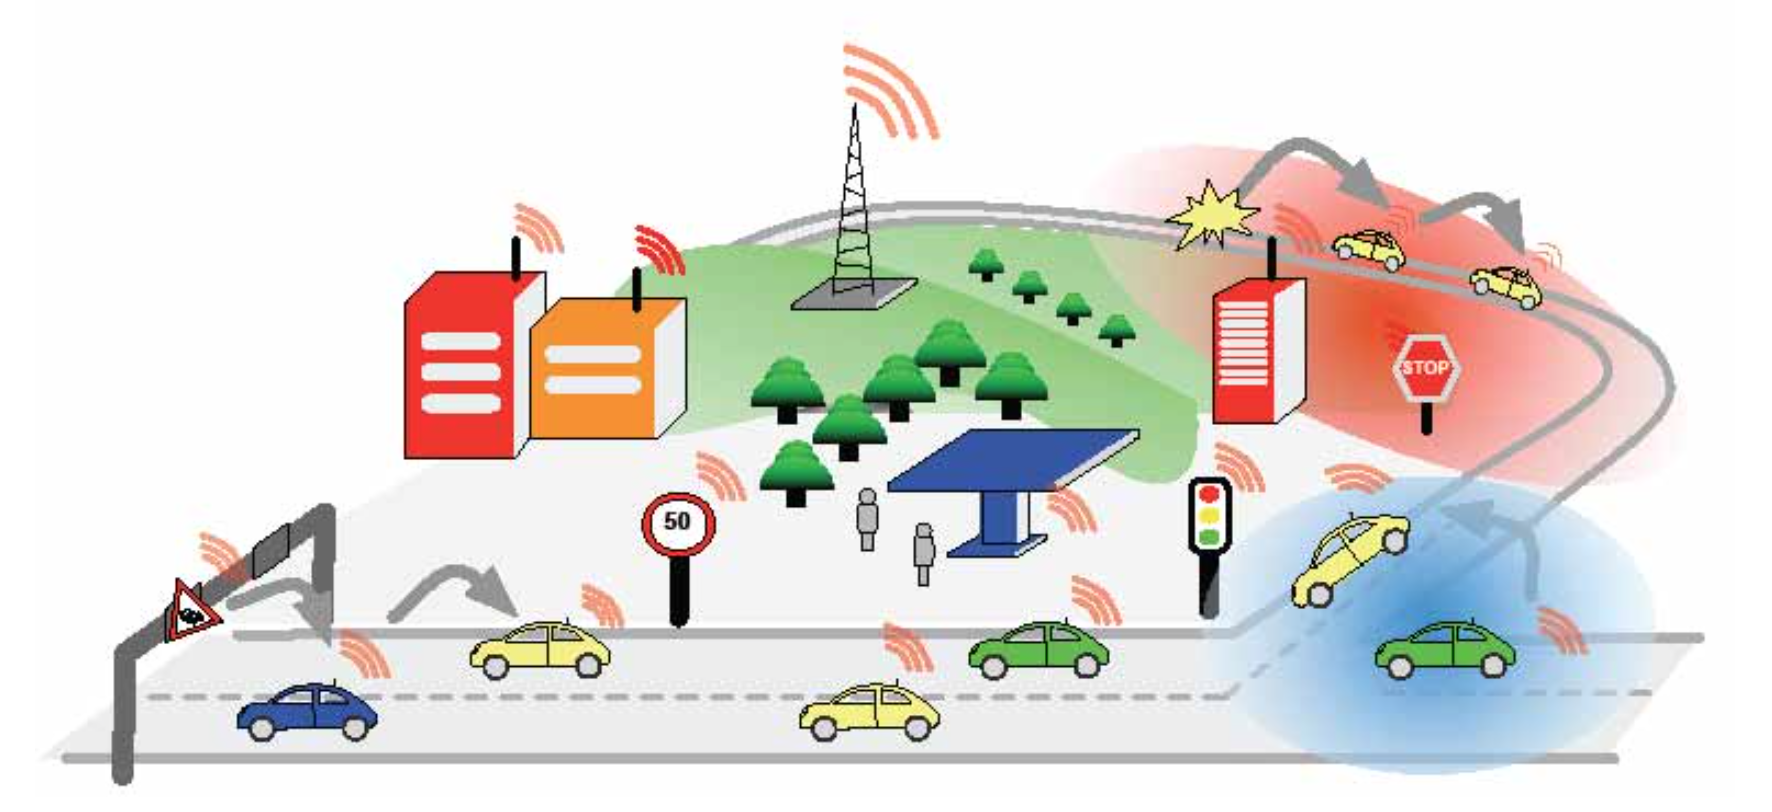
\includegraphics[width=0.99\textwidth]{content/images/06_use_cases/komponenten.png}
\caption{Die Komponenten der \acl{C2C}}
\label{fig:komponentenderc2x}
\end{figure}
Die \acl{C2C} bietet eine große Vielfalt an verschiedenen Einsatzmöglichkeiten. Da es sich bei dem gesamten Projekt nicht nur darum handelt das Fahrzeuge untereinander kommunizieren, sondern wie auf \autoref{fig:komponentenderc2x} zu sehen auch andere Verkehrskomponenten. Hinzu kommt natürlich noch Internet Hotspots die ebenfalls in der C2C eine rolle spielen. Um das Zusammenspiel der Komponenten besser zu verstehen und zu sehen wie groß das Potential der \acl{C2C} ist, werden im folgenden mehrere Szenarien aufgezählt und erklärt. Diese Teilen sich in Sicherheitsbedingte, Verkehrseffiziente und Infotainment ein. 

\section{Sicherheitsbedingt}
Sicherheitsbedingte Szenarien sind Fälle bei denen ein Möglicher Unfall verhindert werden soll. 
\subsection{Cooperative Forward Collision Warning}

\subsection{Pre-Crash Sensing/Warning}

\subsection{Hazardous Location C2C Notification}

\section{Verkehrseffizienz}
\subsection{Enhanced Route Guidance and Navigation}
\subsection{Green Light Optimal Speed Advisory}
\subsection{V2V Merging Assistance}

\section{Infotainment}
\subsection{Internet Access in Vehicle}
\subsection{Point of Interest Notification}
\subsection{Remote Diagnostics}